\documentclass[12pt]{article}
\usepackage{listings}
\usepackage[colorlinks=true,pagebackref,linkcolor=blue]{hyperref}
\usepackage{graphicx}
\textwidth=7in
\textheight=9.5in
\topmargin=-1in
\headheight=0in
\headsep=.5in
\hoffset  -.85in

\lstset{
basicstyle=\footnotesize\ttfamily,
language=bash,
upquote=true,
breakatwhitespace=true,
columns=fullflexible,
keepspaces,
%numbers=none,
tabsize=3,
frame=blrt,
framextopmargin=5pt,
showstringspaces=false,
extendedchars=true
}

\pagestyle{empty}

\renewcommand{\thefootnote}{\fnsymbol{footnote}}

\begin{document}



\begin{center}
{\bf AMS 550.400 \quad HW SET 1\quad  Due Date:  Oct 8}\\
\vskip.2in
{\footnotesize Last Compiled on \today}
\end{center}

\setlength{\unitlength}{1in}

\begin{picture}(6,.1) 
\put(0,0) {\line(1,0){6.25}}         
\end{picture}

 

\renewcommand{\arraystretch}{2}

\noindent\textbf{General Instruction:} 
To complete the homework set, you are required to do the followings. 
Your solutions must be typed in \LaTeX\ using the course homework
template.  
The progression of your homework solution is to be
``recorded'' by making a git folder specifically for this homework
set.  The burden of proof is on you, and if your git commit history
is sparse, then you may be liable for a penalty.  
A paper copy of the PDF output of your \LaTeX\ file is 
to be submitted to your instructor in class on the due date.
\emph{After} submitting the paper copy, but \emph{before} the end of
the due date, you will upload your work to your github by making a remote repository
specifically for the homework, and post the link to the repository 
at the designated \emph{Discussion} forum in Blackboard by making 
a thread just for you.  The repository name in your github should be
\texttt{550400.homeworkset.1} and the discussion forum thread should
be named \texttt{YourFirstNameMiddleInitialLastName}, e.g.,
\texttt{BaracHObama} and \texttt{WillardMRommey}. 
You have till the end of 
the due date to finalize your github repository.  
However, any commit made after the class time of the due date will be 
inadmissible. \emph{Your attention to details in following this instruction will be 
critical, and if not followed exactly at the time of collection, the
homework set may be graded at $90\%$ of the full score}.

\vskip.25in
\noindent\textbf{Problem 1 (10 pts):}  
Assume that you are starting from ``scratch'' at the directory \verb+~/+.
Provide a sequence of git/bash commands that yields a git folder with 
a commit history such that:
\begin{itemize}
\item the \emph{master} branch has commits $A$, $B$, $C$, $X$ and $D$,
\item the \emph{alt} branch has commits $A$, $B$, $X$,
\end{itemize}
Suppose that you are currently working on \texttt{master} branch. Draw 
its commit history graph (i.e., the graph portion of the output of
\verb+git log --graph --oneline+).  Next, assume that 
you are on \texttt{alt} branch. Draw its commit history graph.  

\bigskip
\noindent\textbf{Answer to Problem 1:}\\
Commands:\\
\verb+mkdir problem1.git+\\
\verb+cd problem1.git+\\
\verb+git init .+\\
\verb+vi main.txt+ (Then type A in the content.)\\
\verb+git add .+\\
\verb+git commit -m "A is done"+\\
\verb+vi main.txt+ (Then type B in the content.)\\
\verb+git add .+\\
\verb+git commit -m "B is done"+\\
\verb+git branch alt+\\
\verb+git checkout alt+\\
\verb+vi main.txt+ (Then type X in the content.)\\
\verb+git add .+\\
\verb+git commit -m "X is done"+\\
\verb+git checkout master+\\
\verb+vi main.txt+ (Then type C in the content.)\\
\verb+git add .+\\
\verb+git commit -m "C is done"+\\
\verb+git merge alt+\\
\verb+git commit -a+\\
\verb+vi main.txt+ (Delete the items that don't need and then type D in the content.)\\
\verb+git add .+\\
\verb+git commit -m "D is done"+\\


\noindent{To see its commit history graph on master branch, type in the following command:}\\
\verb+git log --graph --oneline+\\
and the graph is in Figure 1.

\begin{figure}[!htb]
    \begin{center}
        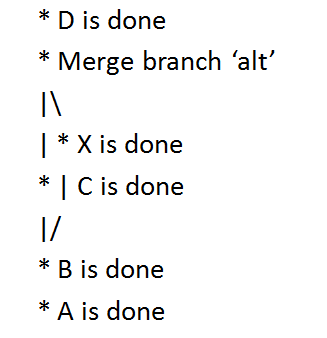
\includegraphics[width=0.75\textwidth]{master.png}
    \end{center}
    \caption{Commit History Graph on Master Branch}
\end{figure}

\noindent{To see the commit history graph on alt branch, type in the following commands:}\\
\verb+git checkout alt+\\
\verb+git log --graph --oneline+\\
and the graph is in Figure 2.

\begin{figure}[!htb]
    \begin{center}
        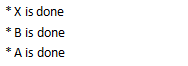
\includegraphics[width=0.5\textwidth]{alt.png}
    \end{center}
    \caption{Commit History Graph on Alt Branch}
\end{figure}

\vskip.25in
\noindent\textbf{Problem 2 (10 pts):}
Assume that you are starting from ``scratch'' at the directory \verb+~/+.
Provide a sequence of git/bash commands that yields a git folder and 
\begin{itemize}
\item configure your git with your name and your email address,
\item set up an alias for each of the git remotes listed below:
\begin{verbatim}
git://github.com/nhlee/550400.stanza1.git 
git://github.com/nhlee/550400.stanza2.git 
git://github.com/nhlee/550400.stanza3.git 
\end{verbatim}
Assume that each remote contains exactly single commit with 
a txt file for a single (different) stanza,
\item pull to combine three stanzas of a poem,
\item after the first pull, add the title of the poem,
\item after the second and third pull, resolve the merge conflict,
\item after resolving the third pull merge conflict, push the result
  to your (newly created) remote repository. 
\end{itemize}

\bigskip
\noindent\textbf{Answer to Problem 2:}\\
To configure my git with my name and email address, type in the following commands:\\
\verb+git config --global user.email xyang39@jhu.edu+\\
\verb+git config --global user.name "Xiaohan Yang"+\\

\noindent{For the stanza, type in the following commands:}\\
\verb+mkdir problem2.git+\\
\verb+cd problem2.git+\\
\verb+git init .+\\
\verb+vi main.txt+ (Then type anything as you like.)\\
\verb+git add .+\\
\verb+git commit -m "beginning"+\\
\verb+git remote add elephant git://github.com/nhlee/550400.stanza1.git+\\
\verb+git pull elephant master+\\
\verb+vi main.txt+ (Delete the items that we don't want and add a title.)\\
\verb+git add .+\\
\verb+git commit -m "stanza1 is done"+\\
\verb+git remote add first git://github.com/nhlee/550400.stanza2.git+\\
\verb+git pull first master+\\
\verb+git commit -a+\\
\verb+vi main.txt+ (Delete the items that we don't need.)\\
\verb+git add .+\\
\verb+git commit -m "stanza2 is done"+\\
\verb+git remote add second git://github.com/nhlee/550400.stanza3.git+\\
\verb+git pull second master+\\
\verb+git commit -a+\\
\verb+vi main.txt+ (Delete the items that we don't need.)\\
\verb+git add .+\\
\verb+git commit -m "stanza3 is done"+\\
\verb+git remote add poem git://github.com/yangxiaohan/550400.homeworkset.1.git+\\
\verb+git push poem master+\\

\newpage
\noindent\textbf{Problem 3 (40 pts):}
Consider a team of four students, say, $A$, $B$, $C$ and $D$, 
who just started working 
on writing a \texttt{latex/beamer} file, say \texttt{main.tex}, 
for a class presentation of their work statement.  
Assume that they do not wish to coordinate their schedules for a
concurrent group meeting (both virtually and physically).  
Assume that:
\begin{itemize}
\item $A$ is in charge of \emph{Introduction},
\item $B$ is of \emph{Problem Statement}, 
\item $C$ is of  \emph{Timeline},
\item $D$ is of \emph{Deliverable} part of the presentation.  
\end{itemize}
In other words, their contributions to \texttt{main.tex} do not overlap.
Then, 
\begin{itemize}
\item first, devise a work flow strategy for the team so that they can
  collaborate asynchronously using \texttt{git},
\item next, devise yet another \texttt{git} strategy different from your earlier
  proposal.  
\end{itemize}
Finally,
\begin{itemize}
\item discuss the strength and weakness of each of your proposed strategies in terms of merge
conflicts resolution,
\item make the final recommendation.  
\end{itemize}
In order to answer this question, \emph{build}
a mathematical model, \emph{following} the guideline from IMM. 
Use Section 1.4 and Section 1.5 of IMM as \emph{role models}.    
For example, you are to identify which variables  are exogenous 
and which are endogenous.  More specifically, among other things, 
in your model, is the preamble part of \texttt{main.tex} an endogenous 
or exogenous variable?  
Note also that in addition to this issue, there are other issues that
you are to consider.  So, \emph{be sure to consult IMM}. 

\newpage
\noindent\textbf{Answer to Problem 3:}\\

One strategy is as the following: each student builds a git folder and does his part under the folder. After finishing his part, he pushes it to his github repository. After all the four students finish their job, one student gets the github addresses of the four students and pull each part from the github repository and merge them. This strategy is illustrated in Figure 3.\\
\begin{figure}[!htb]
    \begin{center}
        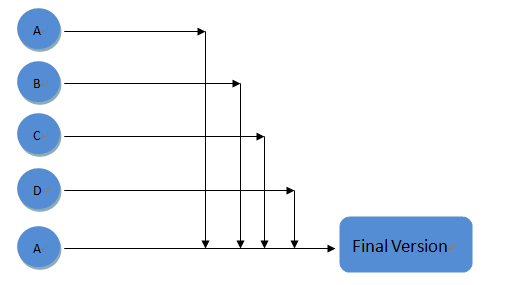
\includegraphics[width=0.6\textwidth]{1.png}
    \end{center}
    \caption{Working Flow of Strategy 1}
\end{figure}

Another strategy is to build a git folder first. Under the folder, build four branches for the four parts. The four students do their own part and push it to their own github repository. Then a student pulls each part from the github repository to the corresponding branch and merges each branch with master branch. This strategy is illustrated in Figure 4.\\
\begin{figure}[!htb]
    \begin{center}
        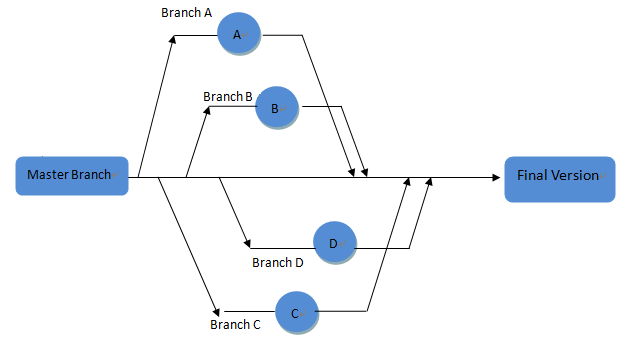
\includegraphics[width=0.78\textwidth]{2.png}
    \end{center}
    \caption{Working Flow of Strategy 2}
\end{figure}

Our problem is to find a better git strategy to combine the work of A, B, C and D so that we can solve merge conflicts well. With the help of git, different people can work separately and more efficiently. After they work out their own parts, they put them together using merge commands in git. But during merging, some problems may arise. So our goal is to develop a strategy that can solve these problems better.\\

To compare the above two strategies, we build a mathematical model. In the model, the way of merging the four parts: introduction, problem statement, timeline and deliverable part of the presentation, and the results of merging are what we want to study, which are the endogenous variables. Other parts of the main.txt file or the presentation, such as the preamble part or the conclusion part of the presentation, are not what we are going to look into, so they are all exogenous variables.\\

If we have a preamble part in the main.txt file, we can commit it before merging. If we have a conclusion part, we can merge one more time, whose procedure is just as the previous merging. So we can simply ignore these two parts and regard the main.txt file as a presentation file made up of only four parts.\\

For the first strategy, suppose student A does the final merging procedure. Then he has to pay attention to each merging step and make sure that he commits before merging otherwise the content will be overwritten. For the second one, the students only need to merge branches A, B, C and D to the master branch. Both methods have to deal with the conflict of merging by deleting the part that is not needed in the main.txt file.\\

The model is useful. The information needed in the model is easy to get and we can make it accurate and satisfying the requirements of the model perfectly. We can let A write the introduction containing only a letter ``A", B write a letter ``B" as the problem statement part, C write ``C" and D write ``D". It takes little effort. Then we merge the four parts according to the two strategies stated above. According to the problems we meet in the merging and how we solve them, we can compare which strategy is better.\\

We get the conclusion that the second strategy is better than the first one from our model. To test the model, we do the simulation procedures. We replace each part by some very simple sentences or even a letter and then merge them to see whether it works better in strategy 2. If yes, then we can say our model is reasonable and in some sense a good model.\\


\newpage
\vskip0.25in
\noindent\textbf{Problem 4 (aka.\ Fair Play, 40 pts):}
Answer the following question:
\begin{verse}
Is the tennis game fair?
\end{verse}
Note that unlike Problem 3, this question is vaguely stated.
This is intensional, whence to begin, you will first need to clarify
what exactly your question is.
You may use the class discussion on this particular 
problem, but you \emph{may not} directly refer to our 
discussion.  Instead, formulate the model carefully but concisely in 
your own words.   

\newpage
\noindent\textbf{Answer to Problem 4:}\\

To build a model to analysis the problem whether the tennis game is fair, we should first fully understand the meaning of the problem. What does fair mean here? In my opinion, it means the fairness of the rules of the game, not the fairness of the umpires or the fairness of anything else. Then how can we say the rules of the tennis game are fair? It is about the probability of win.\\

The rules for a tennis game are complicated. For a whole match, there are several sets and under each set, there are several games. The first player to win two sets in a best-of-three match, or three sets in a best-of-five match, wins the match. To win a set, the player has to win at least six games and at least two games more than the opponent. And for the game, the first player to get at least four points and at least two more points than the opponent wins the game.\\

The server of the first game is decided by a toss before the warm-up starts and after each game, the roles of the server and receiver change. It is accepted by most people that the server has advantage in the game because the serve starts each round of the game and the receiver has to play to the pace of the server. So checking the fairness of the tennis game is equivalent to checking whether the probability of win for the first server changes with the change of the role of the first server. That is, our objective is to answer the following question: if a player is the server in the first game, then does the probability of win for him is the same as the probability in the case where he is not the server in the first game?\\

In our model, we want to explore the relationship between the change of roles and the change of probability of win. The probability of win is also affected by many other factors, such as psychological reasons and the level of skills. Some people may not be good at handling stress, then the probability of win for him may be low although he has good skills. If a player plays much better than the other, it will be much easier for him to win, which means that the probability of win is large. However, because we only want to study whether the rules are fair or not, so the factors stated above are all exogenous variables and we don't discuss them. And even for simplicity, we just assume that the skill levels of the two players are almost the same and the effect of psychological things is trivial. Then if the game is fair, the probability of win for the first server and the first receiver should be the same, which is 0.5. The endogenous variables in our model are the roles of server and receiver and the probability of winning the whole match.\\

If the probability of winning a set for the server of the first game is the same as that for the receiver of the first game, then the two players will have the same probabilities of winning the whole match because it is a best-of three or best-of-five match. So we only need to investigate the probability of winning a set for the server and receiver. Denote $p$ as the probability of winning a game for the server of the game and $P$ as the probability of winning a set for the server of the first game. Then we only need to check whether $P=0.5$. To compute the value of $P$, we first need to collect an enough amount of data, which are the number of sets the two tennis players win in matches with the acknowledge of the first server of each set. And the data should satisfy the following requirements: the two players of the same game should be in the same level of skills and they should not be influenced by other factors such as psychological things.\\

Although the requirements for the data are hard to achieve in real life, the model is still useful because we can make up the data so that they are as close as enough to what we want. To collect data satisfying all the above requirements, we can write a program to simulate the situation. We can set the levels of the two players to be the same in the computer and let the computer play the game. Since we agree with the idea that the server of the game has an advantage over the receiver, we set $p$ to be a number greater than 0.5 and smaller than 1. After thousands of rounds, we count the number of sets one player wins as the server of the first game and the total number of sets that player wins. Then we divide the former number by the latter one to get $P$. If $P$ is close to 0.5, then we conclude that the game is fair, otherwise not.\\

To test the model, we can collect the data from the real life. To make the data as close as possible to the assumptions, we may collect the results of matches between the top two players in the world. The skill levels of the best players in the world should be quite close to each other. And they have taken hundreds of matches so they should not be affected much by mental things. Then we can calculate the probability of winning a set as the server of the first game and get a conclusion to see whether this conclusion agrees with the one we get in our model.\\
 



\newpage
\vskip0.25in
\noindent\textbf{Final Remarks about Problem 3 \& Problem 4:} 
They are open-ended problems.  However, your scores will be determined
by how well do you follow the exposition style outlined by IMM and
WMA.  For both problems, your write-up should be 
\begin{itemize}
\item self-contained,
\item covering all four parts of Section 1.3 of IMM,
\item paying a particular attention to any causal relation that you
  might be investigating, following Chapter 3 of WMA,
\item answering questions that are explicitly asked in the problem statements.
\end{itemize}
For Problem 3, focus mostly on Step 2 and Step 3 of Section
1.3 of IMM.  For Problem 4, focus mostly on Step 1 and Step
2.  For each problem, minimum 1 pages and maximum 2 pages.
\end{document}
